\documentclass{article}
\author{Victor Mittermair, 11809916}
\usepackage{hyperref}
\usepackage{fancyhdr}
\usepackage{tikz} 
\usepackage{amsthm}
\usepackage{verbatim}
\usepackage{subfigure}
\usepackage{amssymb}
\usepackage{mathtools}
\usepackage{amsmath}
\usepackage{soul}
\usepackage{algorithm}
\usepackage{algpseudocode}
\usepackage{algorithmicx}
\usepackage{enumerate}

\newtheorem*{theorem}{Theorem}
\newtheorem*{lemma}{Lemma}
\theoremstyle{definition}
\newtheorem*{definition}{Definition}
\theoremstyle{remark}
\newtheorem*{remark}{Remark}
\newtheorem*{note}{Note}
\newtheorem*{statement}{Statement}
\newtheorem*{example}{Example}

%\lhead{\includegraphics[width=0.2\textwidth]{nyush-logo.pdf}}
\fancypagestyle{firstpage}{%
  \lhead{TU Vienna}
  \rhead{
  Discrete Math for Informatics WS 2022}
}

%%%% PROJECT TITLE
\title{Discrete Math for Informatics\\
        \Large \emph{2nd Lecture}}


\date{\today} %NO DATE

\begin{document}
\maketitle
\thispagestyle{firstpage}

\begin{comment}
\section*{Graph}
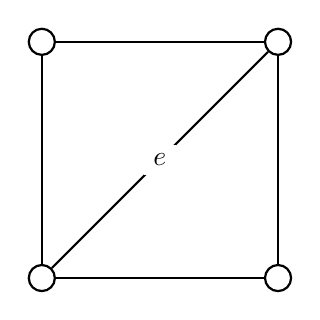
\begin{tikzpicture}[node distance={30mm}, thick, main/.style = {draw, circle}]
    \centering
    \node[main] (1)              {}; 
    \node[main] (2) [right of=1] {};
    \node[main] (3) [below of=1] {}; 
    \node[main] (4) [right of=3] {};
    \draw (1) -- (2) ; 
    \draw (1) -- (3); 
    \draw (2) -- (4); 
    \draw (3) -- (4);
    \draw (3) -- (2) node [midway, fill=white] {$e$}; 
\end{tikzpicture}
\end{comment}


\end{document}